\section{Funciones notables}

\subsection{La función exponencial}

Como la serie $\sum_{n=0}^\infty \frac{z^n}{n!}$ converge absolutamente para todo \(z\in\mathbb{C}\) por el criterio del cociente:
\[
\lim_{n\to\infty} \left|\frac{z^{n+1}/(n+1)!}{z^n/n!}\right| = \lim_{n\to\infty} \frac{|z|}{n+1} = 0 < 1,
\]
tenemos que su radio de convergencia es \(R=\infty\). 

\begin{definición} [Función exponencial compleja]
Definimos la \textbf{función exponencial compleja} como
\[
\begin{matrix}
\exp: \mathbb{C} \to \mathbb{C} \\
     z \mapsto \exp(z) = e^z = \sum_{n=0}^\infty \frac{z^n}{n!}.
\end{matrix}
\]    
\end{definición}


Por las propiedades de las funciones suma de serie de potencias tenemos 

\begin{enumerate}
    \item La función exponencial es de clase $C^\infty$ en todo \(\mathbb{C}\), es decir, es entera.
    \item La derivada de la función exponencial es ella misma: 
    \[
        (exp)'(z) = \sum_{n=1}^\infty \frac{n z^{n-1}}{n!} = \sum_{n=1}^\infty \frac{z^{n-1}}{(n-1)!} = \sum_{m=0}^\infty \frac{z^m}{m!} = exp(z) \quad \forall z \in \mathbb{C}.
    \]
    Con lo cual $(exp)^{(k)}(z) \equiv exp(z)$ para todo \(k\in\mathbb{N}\cup\{0\}\).	
    \item $exp(0) = 1$ y $(exp)^{(k)}(0) = exp(0) = 1 \quad \forall k \in \mathbb{N}\cup\{0\}$.
    
    A partir de aquí, tenemos en cuenta que si $x \in \mathbb{R}$, entonces 
    \[
        exp(x) = \sum_{n=0}^\infty \frac{x^n}{n!} = e^x,
    \]
    escribimos también que $exp(z) = e^z$ para todo \(z\in\mathbb{C}\).
    
    Veamos otras propiedades de la función exponencial.

    \item $exp(z+w) = exp(z)exp(w)$ para todo \(z,w\in\mathbb{C}\). O escrito de otra forma, $e^{z+w} = e^z e^w$.
    \begin{proof}
        Sea $c \in \mathbb{C}$ fijo y definamos la función
        \[
            g(z) = e^{z}e^{c-z} \quad \forall z \in \mathbb{C}.
        \] 
        entoncecs $g$ es derivable y su derivada es
        \[
            g'(z) = e^{z}e^{c-z} + e^{z}e^{c-z}(-1) = 0 \quad \forall z \in \mathbb{C}.
        \]
        \[
            \begin{cases}
                g'(z) = 0 \quad \forall z \in \mathbb{C} \\
                \mathbb{C} \text{ es abierto y conexo}
            \end{cases} \implies g \text{ es constante en } \mathbb{C}.
        \]
        como $g(0) = e^0 e^c = e^c$, tenemos que $g(z) = e^c$ para todo \(z\in\mathbb{C}\). Además, como $c$ es arbitrario, deducimos que $e^{z}e^{c-z} = e^c$ para todo \(z,c\in\mathbb{C}\).\\
        Si ahora tomamos \(c=z+w\), siendo $w\in\mathbb{C}$ arbitrario, obtenemos
        \[
            e^{c} = e^{z+w} = e^{z}e^{c-z} = e^{z}e^{(z+w)-z} = e^{z}e^{w} \quad \forall z,w \in \mathbb{C}.
        \]
    \end{proof}
    \item $exp(z) \neq 0$ para todo \(z\in\mathbb{C}\)
    \begin{proof}
        Si $z \in \mathbb{C}$, como $e^0 = 1$, por la propiedad anterior tenemos que
        \[
            e^z e^{-z} = e^{z + (-z)} = e^0 = 1 \implies e^z \neq 0.
        \]
    \end{proof}
    \item $e^z = e^{x+iy} = e^x(\cos y + i \sin y)$ para todo \(z = x + iy \in \mathbb{C}\) con \(x,y \in \mathbb{R}\).\\
    En efecto,
    \[
        e^{z} = e^{x+iy} = e^x e^{iy} = e^x \left(\sum_{n=0}^\infty \frac{(iy)^n}{n!}\right) = e^x \left(\sum_{n=0}^\infty \frac{i^{2n}y^{2n}}{(2n)!} + \sum_{n=0}^\infty \frac{i^{2n+1}y^{2n+1}}{(2n+1)!}\right).  
    \]
    \[
        = e^x \left(\sum_{n=0}^\infty \frac{(-1)^n y^{2n}}{(2n)!} + i\sum_{n=0}^\infty \frac{(-1)^n y^{2n+1}}{(2n+1)!}\right) = e^x(\cos y + i \sin y).
    \]
    Por tanto, $|e^z| = e^{\Re(z)} \quad \forall z \in \mathbb{C}$ y $|e^{iy}| = 1 \quad \forall y \in \mathbb{R}$.
    \item $exp$ es periódica de periodo $2\pi i$, es decir, $e^{z + 2k\pi i} = e^z$ para todo \(z \in \mathbb{C}\) y todo \(k \in \mathbb{Z}\).
    \begin{proof}
        En efecto,
        \[
            e^{z + 2k\pi i} = e^z e^{2k\pi i} = e^z(\cos(2k\pi) + i \sin(2k\pi)) = e^z(1 + 0) = e^z.
        \]
    \end{proof}
\end{enumerate}

Veamos en qué transforma esta función algunos subconjuntos de $\mathbb{C}$.

\begin{itemize}
    \item \[
    exp\{x : x \in \mathbb{R}\} = \{e^x : x \in \mathbb{R}\} = (0, \infty) 
    \]
    es la semirrecta positiva del eje real.
    
    \begin{center}
    \begin{tikzpicture}[scale=0.8]
        % Conjunto de partida
        \begin{scope}[xshift=-6cm]
            \draw[->, thick] (-2,0) -- (2,0) node[right] {$\Re$};
            \draw[->, thick] (0,-1.5) -- (0,1.5) node[above] {$\Im$};
            \draw[red, very thick] (-1.5,0) -- (1.5,0);
            \node[below] at (0,-1.8) {Conjunto: $\{x : x \in \mathbb{R}\}$};
        \end{scope}
        
        % Flecha
        \draw[->, very thick] (-2.5,0) -- (-1.5,0) node[midway, above] {$\exp$};
        
        % Imagen
        \begin{scope}[xshift=4cm]
            \draw[->, thick] (-1,0) -- (3,0) node[right] {$\Re$};
            \draw[->, thick] (0,-1.5) -- (0,1.5) node[above] {$\Im$};
            \draw[blue, very thick] (0.1,0) -- (2.5,0);
            \filldraw[blue] (0,0) circle (1pt);
            \node[below] at (1,-1.8) {Imagen: $(0,\infty)$};
        \end{scope}
    \end{tikzpicture}
    \end{center}
    
    \item \[
    exp(\{x + iy_0 : x \in \mathbb{R}\}) = \{e^{x}(\cos y_0 + i \sin y_0) : x \in \mathbb{R}\}
    \]
    es la semirrecta que parte del origen y forma un ángulo $y_0$ con el eje real positivo.
    
    \begin{center}
    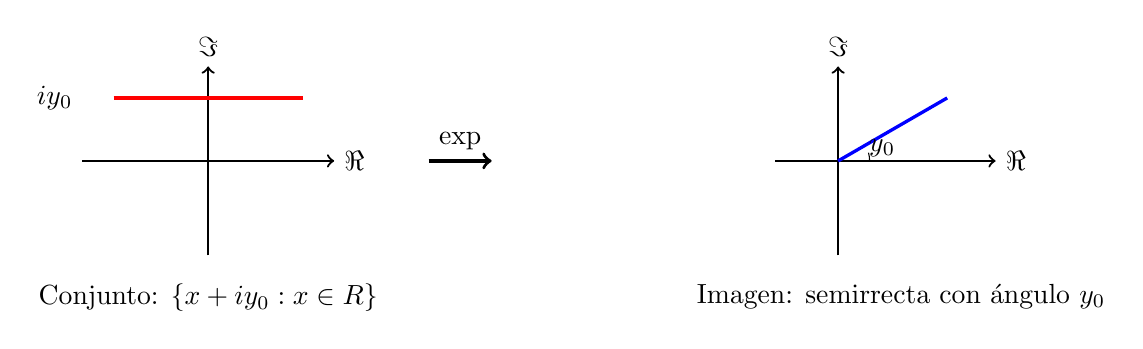
\begin{tikzpicture}[scale=0.8]
        % Conjunto de partida
        \begin{scope}[xshift=-6cm]
            \draw[->, thick] (-2,0) -- (2,0) node[right] {$\Re$};
            \draw[->, thick] (0,-1.5) -- (0,1.5) node[above] {$\Im$};
            \draw[red, very thick] (-1.5,1) -- (1.5,1);
            \node[left] at (-2,1) {$iy_0$};
            \node[below] at (0,-1.8) {Conjunto: $\{x + iy_0 : x \in \mathbb{R}\}$};
        \end{scope}
        
        % Flecha
        \draw[->, very thick] (-2.5,0) -- (-1.5,0) node[midway, above] {$\exp$};
        
        % Imagen
        \begin{scope}[xshift=4cm]
            \draw[->, thick] (-1,0) -- (2.5,0) node[right] {$\Re$};
            \draw[->, thick] (0,-1.5) -- (0,1.5) node[above] {$\Im$};
            \draw[blue, very thick] (0,0) -- ({2*cos(30)},{2*sin(30)});
            \draw[dashed] (0.5,0) arc (0:30:0.5);
            \node at (0.7,0.2) {$y_0$};
            \node[below] at (1,-1.8) {Imagen: semirrecta con ángulo $y_0$};
        \end{scope}
    \end{tikzpicture}
    \end{center}
    
    \item \[
    exp(\{iy : y \in \mathbb{R}\}) = \{e^{iy} : y \in \mathbb{R}\} = \{\cos y + i \sin y : y \in \mathbb{R}\}
    \]
    es la circunferencia unidad centrada en el origen.
    
    \begin{center}
    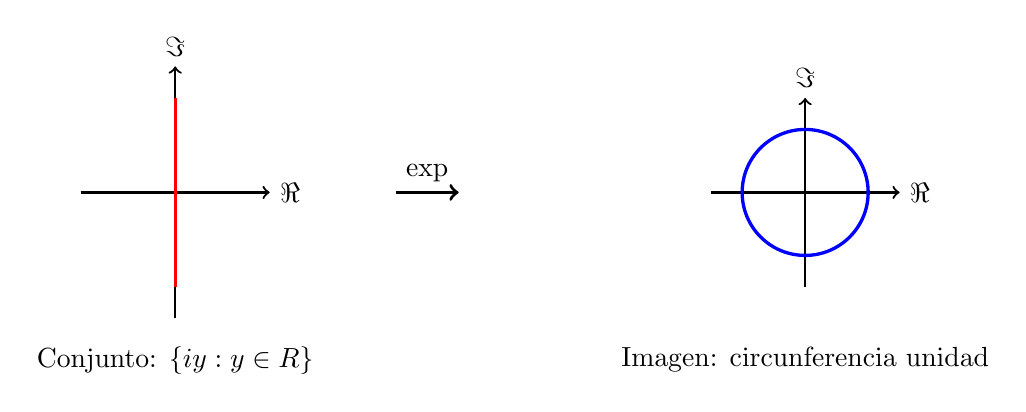
\begin{tikzpicture}[scale=0.8]
        % Conjunto de partida
        \begin{scope}[xshift=-6cm]
            \draw[->, thick] (-1.5,0) -- (1.5,0) node[right] {$\Re$};
            \draw[->, thick] (0,-2) -- (0,2) node[above] {$\Im$};
            \draw[red, very thick] (0,-1.5) -- (0,1.5);
            \node[below] at (0,-2.3) {Conjunto: $\{iy : y \in \mathbb{R}\}$};
        \end{scope}
        
        % Flecha
        \draw[->, very thick] (-2.5,0) -- (-1.5,0) node[midway, above] {$\exp$};
        
        % Imagen
        \begin{scope}[xshift=4cm]
            \draw[->, thick] (-1.5,0) -- (1.5,0) node[right] {$\Re$};
            \draw[->, thick] (0,-1.5) -- (0,1.5) node[above] {$\Im$};
            \draw[blue, very thick] (0,0) circle (1);
            \node[below] at (0,-2.3) {Imagen: circunferencia unidad};
        \end{scope}
    \end{tikzpicture}
    \end{center}
    
    \item
    \[
        exp(\{a + iy : y \in \mathbb{R}\}) = \{e^{a}(\cos y + i \sin y) : y \in \mathbb{R}\} = \{z \in \mathbb{C} : |z| = e^a\}
    \]
    es la circunferencia de radio $e^a$ centrada en el origen.
    
    \begin{center}
    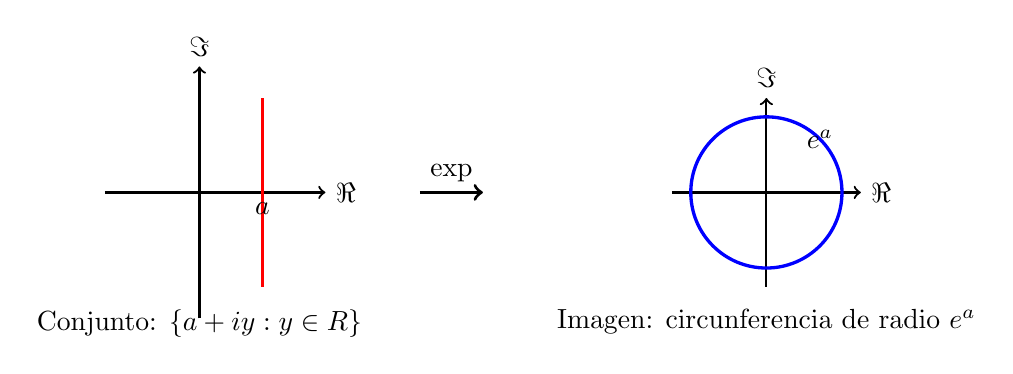
\begin{tikzpicture}[scale=0.8]
        % Conjunto de partida
        \begin{scope}[xshift=-6cm]
            \draw[->, thick] (-1.5,0) -- (2,0) node[right] {$\Re$};
            \draw[->, thick] (0,-2) -- (0,2) node[above] {$\Im$};
            \draw[red, very thick] (1,-1.5) -- (1,1.5);
            \node[below] at (1,0) {$a$};
            \node[below] at (0,-1.7) {Conjunto: $\{a + iy : y \in \mathbb{R}\}$};
        \end{scope}
        
        % Flecha
        \draw[->, very thick] (-2.5,0) -- (-1.5,0) node[midway, above] {$\exp$};
        
        % Imagen
        \begin{scope}[xshift=3cm]
            \draw[->, thick] (-1.5,0) -- (1.5,0) node[right] {$\Re$};
            \draw[->, thick] (0,-1.5) -- (0,1.5) node[above] {$\Im$};
            \draw[blue, very thick] (0,0) circle (1.2);
            \node at (0.85,0.85) {$e^a$};
            \node[below] at (0,-1.7) {Imagen: circunferencia de radio $e^a$};
        \end{scope}
    \end{tikzpicture}
    \end{center}
    
    \item \[
        exp(\{ x + iy : a < x < b, y \in \mathbb{R}\}) = \{e^{x}(\cos y + i \sin y) : a < x < b, y \in \mathbb{R}\} = \{z \in \mathbb{C} : e^a < |z| < e^b\}
    \]
    es el anillo centrado en el origen con radios $e^a$ y $e^b$.
    
    \begin{center}
    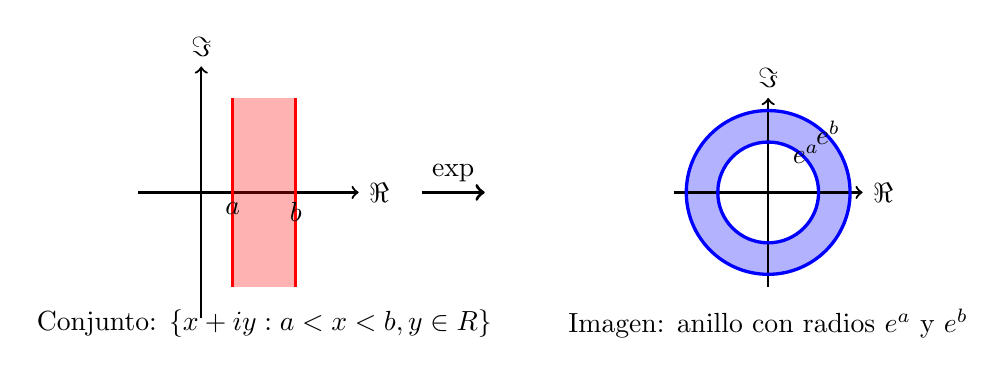
\begin{tikzpicture}[scale=0.8]
        % Conjunto de partida
        \begin{scope}[xshift=-6cm]
            \draw[->, thick] (-1,0) -- (2.5,0) node[right] {$\Re$};
            \draw[->, thick] (0,-2) -- (0,2) node[above] {$\Im$};
            \fill[red, opacity=0.3] (0.5,-1.5) rectangle (1.5,1.5);
            \draw[red, very thick] (0.5,-1.5) -- (0.5,1.5);
            \draw[red, very thick] (1.5,-1.5) -- (1.5,1.5);
            \node[below] at (0.5,0) {$a$};
            \node[below] at (1.5,0) {$b$};
            \node[below] at (1,-1.7) {Conjunto: $\{x + iy : a < x < b, y \in \mathbb{R}\}$};
        \end{scope}
        
        % Flecha
        \draw[->, very thick] (-2.5,0) -- (-1.5,0) node[midway, above] {$\exp$};
        
        % Imagen
        \begin{scope}[xshift=3cm]
            \fill[blue, opacity=0.3] (0,0) circle (1.3);
            \fill[white] (0,0) circle (0.8);
            \draw[->, thick] (-1.5,0) -- (1.5,0) node[right] {$\Re$};
            \draw[->, thick] (0,-1.5) -- (0,1.5) node[above] {$\Im$};
            \draw[blue, very thick] (0,0) circle (0.8);
            \draw[blue, very thick] (0,0) circle (1.3);
            \node at (0.6,0.6) {$e^a$};
            \node at (0.95,0.95) {$e^b$};
            \node[below] at (0,-1.7) {Imagen: anillo con radios $e^a$ y $e^b$};
        \end{scope}
    \end{tikzpicture}
    \end{center}
\end{itemize}

\subsection{Las funciones seno y coseno}

Definimos 

\[
    \sin(z) = \sum_{n=0}^{\infty} (-1)^n \frac{z^{2n+1}}{(2n+1)!}, \quad z \in \mathbb{C} \qquad \text{y} \qquad \cos(z) = \sum_{n=0}^{\infty} (-1)^n \frac{z^{2n}}{(2n)!}, \quad z \in \mathbb{C}.
\]

La definición está bien definidad, pues el radio de convergencia de ambas series es infinito, como se puede comprobar usando el criterio del cociente.

Por las proposiciones de las funciones suma de series de potencias

\begin{itemize}
    \item $\sin(z)$ y $\cos(z)$ son holomorfas en $\mathbb{C}$ y además infinitamente derivables en $\mathbb{C}$. También se cumple que
    \[
        \sin'(z) = \sum_{n=0}^{\infty} (-1)^n \frac{(2n+1)z^{2n}}{(2n+1)!} = \sum_{n=0}^{\infty} (-1)^n \frac{z^{2n}}{(2n)!} = \cos(z),
    \]
    \[
        \cos'(z) = \sum_{n=0}^{\infty} (-1)^n \frac{(2n)z^{2n-1}}{(2n)!} = \sum_{n=1}^{\infty} (-1)^{n} \frac{z^{2n-1}}{(2n-1)!} \underbrace{=}_{m=n+1 \implies n=m-1} \sum_{m=0}^{\infty} (-1)^{m+1} \frac{z^{2m+1}}{(2m+1)!}
    \]

    \[
        = -\sum_{m=0}^{\infty} (-1)^m \frac{z^{2m+1}}{(2m+1)!} = -\sin(z).
    \]
\end{itemize}

Sea $z \in \mathbb{C}$,

\[
    e^{iz} = \sum_{n=0}^{\infty} \frac{(iz)^n}{n!} = \sum_{n=0}^{\infty} \frac{i^{2n}}{(2n)!} + \sum_{n=0}^{\infty} \frac{(iz)^{2n+1}}{(2n+1)!} 
\]

\[
    = \sum_{n=0}^{\infty} \frac{{}(i^2)^n z^{2n}}{(2n)!} + \sum_{n=0}^{\infty} \frac{i^{n} i z^{2n+1}}{(2n+1)!} = \sum_{n=0}^{\infty} (-1)^n \frac{z^{2n}}{(2n)!} + i\sum_{n=0}^{\infty} (-1)^n \frac{z^{2n+1}}{(2n+1)!} = \cos(z) + i\sin(z).	
\]

Luego 

\[
    e^{iz} = \cos(z) + i\sin(z) \quad \forall z \in \mathbb{C}.
\]

\begin{definición}[Funciones seno y coseno complejas]
    Por la definición es claro que $\cos(-z) = \cos(z)$ y $\sin(-z) = -\sin(z)$, para todo $z \in \mathbb{C}$. 

\[
    \begin{cases}
        e^{iz} = \cos(z) + i\sin(z) \\
        e^{-iz} = \cos(-z) + i\sin(-z) = \cos(z) - i\sin(z)
    \end{cases} \implies \begin{cases}
        \cos(z) = \frac{1}{2}(e^{iz} + e^{-iz}) \\
        \sin(z) = \frac{1}{2i}(e^{iz} - e^{-iz})
    \end{cases} \quad \forall z \in \mathbb{C}.
\]  

Así, las funciones seno y coseno complejas se pueden definir también como:

\[
\cos(z) = \frac{e^{iz} + e^{-iz}}{2}
\quad \forall z \in \mathbb{C}.
\]
\[
\sin(z) = \frac{e^{iz} - e^{-iz}}{2i}
\quad \forall z \in \mathbb{C}.
\]

\end{definición}

\begin{proposición}
    Para todo $z,w \in \mathbb{C}$ se cumple que
    \begin{enumerate}
        \item $\cos^2(z) + \sin^2(z) = 1$.
        \item $\sin(z+w) = \sin(z)\cos(w) + \cos(z)\sin(w)$.
        \item $\cos(z+w) = \cos(z)\cos(w) - \sin(z)\sin(w)$.
    \end{enumerate}
\end{proposición}

\begin{proof}
    \leavevmode
    \begin{enumerate}
        \item \[
            \sin^2(z) + \cos^2(z) = \left(\frac{e^{iz} - e^{-iz}}{2i}\right)^2 + \left(\frac{e^{iz} + e^{-iz}}{2}\right)^2 
        \]
        \[
            = \frac{(e^{iz} - e^{-iz})^2}{-4} + \frac{(e^{iz} + e^{-iz})^2}{4} = \frac{-(e^{2iz} - 2 + e^{-2iz}) + (e^{2iz} + 2 + e^{-2iz})}{4} = 1.
        \]
        \item \[
            \sin(z)\cos(w) + \cos(z)\sin(w) = \frac{e^{iz} - e^{-iz}}{2i} \cdot \frac{e^{iw} + e^{-iw}}{2} + \frac{e^{iz} + e^{-iz}}{2} \cdot \frac{e^{iw} - e^{-iw}}{2i}
        \]
        \[
            = \frac{1}{4i} \left( (e^{iz} - e^{-iz})(e^{iw} + e^{-iw}) + (e^{iz} + e^{-iz})(e^{iw} - e^{-iw}) \right)
        \]
        \[
            = \frac{1}{4i} \left( e^{i(z+w)} + e^{i(z-w)} - e^{-i(z-w)} - e^{-i(z+w)} + e^{i(z+w)} - e^{i(z-w)} + e^{-i(z-w)} - e^{-i(z+w)} \right)
        \]
        \[
            = \frac{1}{4i} \left( 2e^{i(z+w)} - 2e^{-i(z+w)} \right) = \frac{e^{i(z+w)} - e^{-i(z+w)}}{2i} = \sin(z+w).
        \]
        \item \[
            \cos(z)\cos(w) - \sin(z)\sin(w) = \frac{e^{iz} + e^{-iz}}{2} \cdot \frac{e^{iw} + e^{-iw}}{2} - \frac{e^{iz} - e^{-iz}}{2i} \cdot \frac{e^{iw} - e^{-iw}}{2i}
        \]
        \[
            = \frac{1}{4} \left( (e^{iz} + e^{-iz})(e^{iw} + e^{-iw}) - (e^{iz} - e^{-iz})(e^{iw} - e^{-iw}) \right)
        \]
        \[
            = \frac{1}{4} \left( e^{i(z+w)} + e^{i(z-w)} + e^{-i(z-w)} + e^{-i(z+w)} - e^{i(z+w)} + e^{i(z-w)} + e^{-i(z-w)} - e^{-i(z+w)} \right)
        \]
        \[
            = \frac{1}{4} \left( 2e^{i(z-w)} + 2e^{-i(z-w)} \right) = \frac{e^{i(z-w)} + e^{-i(z-w)}}{2} = \cos(z+w).
        \]
    \end{enumerate}
\end{proof}

\begin{itemize}
    \item Las funciones seno y coseno son periódicas de periodo $2\pi$, es decir, $\sin(z + 2k\pi) = \sin(z)$ y $\cos(z + 2k\pi) = \cos(z)$ para todo \(z \in \mathbb{C}\) y todo \(k \in \mathbb{Z}\).

    En efecto

    \[
        \cos(z+2\pi) =\cos(z)\underbrace{\cos(2\pi)}_{1} - \sin(z)\underbrace{\sin(2\pi)}_{0} = \cos(z), \quad \forall z \in \mathbb{C},
    \]
    \item Las funciones seno y coseno no son acotadas en \(\mathbb{C}\).\\
    Sea $y > 0$, entonces
    \[
        |\sin(iy)| = \left|\frac{e^{-y} - e^{y}}{2i}\right| = \left|\frac{e^{y} - e^{-y}}{2}\right| = \frac{1}{2} \left(e^{y} - e^{-y}\right) = \frac{1}{2} \left(e^y - \frac{1}{e^y}\right) \xrightarrow{y \to \infty} \infty,
    \]
    Por lo tanto $\sin$ no es acotada en \(\mathbb{C}\). De forma análoga se demuestra que $\cos$ no es acotada en \(\mathbb{C}\).
    \item Los ceros de $\sin$ y $\cos$ son respectivamente los de $\sin(x)$ y $\cos(x)$, es decir,
    \[
        \{z \in \mathbb{C} : \sin(z) = 0\} = \{x \in \mathbb{R} : \sin(x) = 0\} = \{k\pi : k \in \mathbb{Z}\},
    \]
    \[
        \{z \in \mathbb{C} : \cos(z) = 0\} = \{x \in \mathbb{R} : \cos(x) = 0\} = \left\{\frac{\pi}{2} + k\pi : k \in \mathbb{Z}\right\}.
    \]
    En efecto,
    \[
        0 = \sin(z) = \frac{e^{iz} - e^{-iz}}{2i} \underbrace{=}_{z=x+iy} \frac{e^{i(x+iy)} - e^{-i(x+iy)}}{2i} = \frac{e^{ix}e^{-y} - e^{-ix}e^{y}}{2i}
    \]
    \[
        \iff e^{-y}(\cos (x) + i \sin (x)) - e^{y}(\cos (-x) - i \sin (-x)) = 0
    \]
    \[
        \iff e^{-y}(\cos (x) + i \sin (x)) - e^{y}(\cos (x) + i \sin (x)) = 0
    \]
    \[
        \iff e^{-y}(\cos (x) + i \sin (x)) = e^{y}(\cos (x) + i \sin (x)).
        \iff \begin{cases}
        e^{-y} = e^{y} \\
        \cos (x) + i \sin (x) = \cos(-x) + i \sin(-x)
    \end{cases}
    \]
    \[
        \iff \begin{cases}
            -y = y \\
            \cos (x) + i \sin (x) = \cos(x) - i \sin(x)
        \end{cases} \iff \begin{cases}
            y = 0 \\
            \sin(x) = 0
        \end{cases}
    \]
    \[
        \iff \begin{cases}
            z = x + iy = x \\
            \sin(x) = 0
        \end{cases}
    \]
\end{itemize}

\begin{definición}[Funciones trigonométricas]
    La \textbf{función tangente} se define como
    \[
        \tan(z) = \frac{\sin(z)}{\cos(z)} \quad \forall z \in \mathbb{C} \setminus \left\{\frac{\pi}{2} + k\pi : k \in \mathbb{Z}\right\}.
    \]
    Asimismo, la \textbf{función cotangente} se define como
    \[
        \cot(z) = \frac{\cos(z)}{\sin(z)} \quad \forall z \in \mathbb{C} \setminus \{k\pi : k \in \mathbb{Z}\}.
    \]
    La \textbf{función secante} se define como
    \[
        \sec(z) = \frac{1}{\cos(z)} \quad \forall z \in \mathbb{C} \setminus \left\{\frac{\pi}{2} + k\pi : k \in \mathbb{Z}\right\}.
    \]
    Y la \textbf{función cosecante} se define como
    \[
        \csc(z) = \frac{1}{\sin(z)} \quad \forall z \in \mathbb{C} \setminus \{k\pi : k \in \mathbb{Z}\}.
    \]
\end{definición}

También se define las siguientes funciones:
\begin{definición}[Funciones hiperbólicas]
    Definimos las funciones \textbf{seno hiperbólico} y \textbf{coseno hiperbólico} como
    \[
        \sinh(z) = \frac{e^z - e^{-z}}{2} \quad \forall z \in \mathbb{C}, \qquad \cosh(z) = \frac{e^z + e^{-z}}{2} \quad \forall z \in \mathbb{C}.
    \]
\end{definición}

Resulta que 

\[
    \cosh(z) = \cos(iz), \quad \sinh(z) = -i\sin(iz) \quad \forall z \in \mathbb{C}.
\]

\subsection{La función logaritmo complejo}

En $R$ la función $e^x$ es inyectiva, luego tiene inversa, que es la función logaritmo natural, denotada por $\ln(x)$. En $\mathbb{C}$ la función $e^z$ no es inyectiva, luego no tiene inversa, es decir, si $z \in \mathbb{C} \setminus \{0\}$, entonces existen infinitos $w \in \mathbb{C}$ tales que $e^w = z$, de la siguiente forma:
\[
z = |z|(\cos(\theta) + i\sin(\theta)) \text{ con } \theta = \arg(z)
\]
\[
e^w = z \iff e^{a+bi} = |z|(\cos(\theta) + i\sin(\theta)) \iff e^a(\cos(b) + i\sin(b)) = |z|(\cos(\theta) + i\sin(\theta)) \iff
\]
\[
\begin{cases}
e^a = |z| \\
\cos(b) = \cos(\theta) \\
\sin(b) = \sin(\theta)
\end{cases} \iff \begin{cases}
a = \ln|z| \\
b = \theta + 2k\pi, \quad k \in \mathbb{Z}
\end{cases}
\iff
w = \ln|z| + i(\theta + 2k\pi), \quad k \in \mathbb{Z}
\]

Es mas, la banda $\{ w = a + bi : a \in \mathbb{R}, b \in [0, 2\pi) \}$ genera todo $\mathbb{C} \setminus \{0\}$ mediante la función exponencial, es decir,
\[
    \exp(\{ w = a + bi : a \in \mathbb{R}, b \in [0, 2\pi) \}) = \mathbb{C} \setminus \{0\}.
\]

Y esto mismo ocurre para cualquier banda de longitud $2\pi$, es decir, si $\alpha \in \mathbb{R}$, entonces
\[
    \exp(\{ w = a + bi : a \in \mathbb{R}, b \in (\alpha, \alpha + 2\pi] \}) = \mathbb{C} \setminus \{0\}.
\]

\begin{definición}
    Así si $z \in \mathbb{C} \setminus \{0\}$ tenemos que:
\[
    \{ w \in \mathbb{C} : e^w = z \} = 
    \{\ln|z| + i(\theta + 2k\pi) : k \in \mathbb{Z}\}.
\]
A cada elemento del conjunto se dice que es un \textbf{logaritmo complejo} de $z$.
Si restringimos el argumento de $z$ a un intervalo de longitud $2\pi$, como puede ser $(-\pi, \pi]$, tenemos entonces un único $w \in \mathbb{C}$ tal que $e^w = z$, y a este $w$ se le llama el \textbf{logaritmo principal} de $z$:
\[
    \text{Log}(z) = \ln|z| + i\theta, \quad 
    \begin{cases}
        \forall z = |z|(\cos(\theta) + i\sin(\theta)) \in \mathbb{C} \setminus \{0\} \\
        \theta = \arg(z) \in (-\pi, \pi]
    \end{cases}
\]
\end{definición}

En general si $\alpha \in \mathbb{R}$, denotamos por $\text{Log}_\alpha(z)$ a la función:
\[
    \text{Log}_\alpha(z) = \ln|z| + i\theta, \quad 
    \begin{cases}
        \forall z = |z|(\cos(\theta) + i\sin(\theta)) \in \mathbb{C} \setminus \{0\} \\
        \theta = \arg(z) \in (\alpha, \alpha + 2\pi]
    \end{cases}
\]

Ahora, si $\Omega \in \mathbb{C}$ es un abierto conexo y $f : \Omega \to \mathbb{C}$ cumple que es continua y $e^{f(z)} = z \quad \forall z \in \Omega$, diremos entonces que $f$ es una \textbf{determinacion continua de $\log(z)$ en $\Omega$}, o tambien que $f$ es una \textbf{rama de $\log(z)$ en $\Omega$}.\\
De esta forma cada $f_\alpha = \log_\alpha$ es una rama de $\log(z)$.\\

Para tener una determinación continua de $\log(z)$ es necesario y suficiente tener una determinación continua del argumento de $z$.\\
El argumento principal es una determinación no continua del argumento:
\[
    Arg : \mathbb{C} \setminus \{0\} \to (-\pi, \pi]
\]
Ya que $\nexists \lim_{z \to -1} Arg(z)$, pues
\[    \lim_{z \to -1, z \in \text{semirrecta superior}} Arg(z) = \pi, \quad \lim_{z \to -1, z \in \text{semirrecta inferior}} Arg(z) = -\pi.
\]

\begin{proposición}
    Sea $\Omega \subset \mathbb{C} \setminus \{0\}$ un abierto conexo y sea $f : \Omega \to \mathbb{C}$ una determinación continua del logaritmo, entonces $f$ es holomorfa en $\Omega$ y:
    \[
        f'(z) = \frac{1}{z} \quad \forall z \in \Omega.
    \]
\end{proposición}

\begin{proof}
    Sea $z_0 \in \Omega$, entonces debemos comprobar:
    \[
        f'(z_0) = \lim_{z \to z_0} \frac{f(z) - f(z_0)}{z - z_0} = 
        \lim_{z \to z_0} \frac{\log(z) - \log(z_0)}{z - z_0} = 
        \frac{1}{z_0}
    \]
    Sabemos que $e^{f(z)} = z \quad \forall z \in \Omega$, luego podemos tomar una sucesión $(z_n)_{n=1}^\infty\subset \Omega \setminus \{z_0\}$ tal que $z_n \to z_0$. Llamemos además $w_0 = f(z_0)$ y $w_n = f(z_n) \quad \forall n \in \mathbb{N}$. Entonces:
    \[
    \frac{f(z_n) - f(z_0)}{z_n - z_0} =
    \frac{w_n - w_0}{z_n - z_0} =
    \frac{w_n - w_0}{e^{f(z_n)} - e^{f(z_0)}} =
    \frac{1}{\frac{e^{f(z_n)} - e^{f(z_0)}}{w_n - w_0}} =
    \frac{1}{\frac{e^{w_n} - e^{w_0}}{w_n - w_0}}
    \longrightarrow^{n \to \infty} \frac{1}{e^{w_0}} = \frac{1}{z_0}
    \]
    Por tanto:
    \[
        f'(z_0) = \lim_{n \to \infty} \frac{f(z_n) - f(z_0)}{z_n - z_0} = \frac{1}{z_0}.
    \]
\end{proof}

\begin{observación}
    $\log$ es holomorfa en:
    \[
    \mathbb{C} \setminus \{z \in \mathbb{C} : \Re(z) \leq 0, \Im(z) = 0\} =
    \mathbb{C} \setminus (-\infty, 0]
    \]
    Es decir, en $\mathbb{C}$ menos el eje real negativo y el origen.\\
\end{observación}

\begin{observación}
    En general, al estar en $\mathbb{C}$ no se cumple que:
    \[
        \log(zw) = \log(z) + \log(w)
    \]
    Por ejemplo:
    \[
    \log(i) = \ln|i| + i\frac{\pi}{2} = i\frac{\pi}{2}, \quad
    \log(-i) = \ln|-i| + i\left(-\frac{\pi}{2}\right) = -i\frac{\pi}{2}
    \]
    \[
        \log(i) + \log(-i) = i\frac{\pi}{2} - i\frac{\pi}{2} = 0 \neq \log(i \cdot -i) = \log(1) = 0
    \]
    Pero $\log(i) + \log(-i) = 0 + 2\pi i = \log(1)$.\\
    Otra cosa a tener en cuenta es que $e^{\log(z)} = z \quad \forall z \in \mathbb{C} \setminus \{0\}$, pero $\log(e^z) \neq z \quad \forall z \in \mathbb{C}$.
\end{observación}

\subsection{La función potencia compleja}

Dado $\alpha \in \mathbb{C}$ queremos definir $z^\alpha$ para $z \in \mathbb{C} \setminus \{0\}$.\\
Podemos definir:
\[
\begin{cases}
    z^\alpha = \\
    e^{\alpha \log(z)} = \\
    e^{\alpha \log(z)} : \log(z) \text{ es cualquier logaritmo complejo de } z = \\
    e^{\alpha (\ln|z| + i(\theta))} : \theta = \arg(z)
\end{cases}
\]

Que puede tener solo un elemento si $\alpha \in \mathbb{Z}$, numerables si $\alpha \in \mathbb{Q}$ y no numerables si $\alpha \in \mathbb{C} \setminus \mathbb{R}$.\\


Queremos saber cuantos valores puede tomar $z^\alpha$:
\begin{itemize}
    \item Si $\alpha = 0$ entonces $e^{\alpha \log(z)} = e^0 = 1 \quad \forall z \in \mathbb{C} \setminus \{0\}$.
    \item Si $\alpha = n \in \mathbb{N}$, sea $\theta_0 = \arg(z)$, entonces los argumentos de $z$ son $\theta_k = \theta_0 + 2k\pi, k \in \mathbb{Z}$, luego: 
    \[
    e^{\alpha \log(z)} = 
    e^{\alpha(\ln|z| + (\theta_0 + 2k\pi)i)} =
    e^{\alpha \ln|z|} e^{\alpha (\theta_0 + 2k\pi)i} = 
    \left(e^{\ln|z|}\right)^\alpha \left(\cos(\alpha \theta_0 + 2k\alpha \pi) + i\sin(\alpha \theta_0 + 2k\alpha \pi)\right) =
    \]
    \[
    |z|^\alpha \left(\cos(\alpha \theta_0 + 2k\alpha \pi) + i\sin(\alpha \theta_0 + 2k\alpha \pi)\right) =_{\alpha \in \mathbb{N}}
    |z|^n \left( \cos (n\theta_0) + i \sin (n\theta_0) \right) =
    z^n \quad \forall k \in \mathbb{Z}
    \]
    \item Si $\alpha = -n: n \in \mathbb{N}$, entonces:
    \[
    z^\alpha = z^{-n} = \frac{1}{z^n} \quad \forall z \in \mathbb{C} \setminus \{0\}
    \]
    Así, si $p \in \mathbb{Z}$, entonces $z^p$ tiene un único valor para todo $z \in \mathbb{C} \setminus \{0\}$.
    \item Si $\alpha = p = \frac{1}{n} : \quad n \in \mathbb{N}$ tenemos que $z^p=z^{\frac{1}{n}}$ tiene $n$ valores, asociados a cada raiz $n-sima$.
    \item Si $\alpha = \frac{p}{q} \in \mathbb{Q}$ con $p,q$ coprimos entre si, tenemos que:
    \[
    z^\alpha = z^{\frac{p}{q}} = \left(z^{\frac{1}{q}}\right)^p
    \]
    Que por lo antes visto nos da $q$ resultados distintos.
    \item Si $\alpha \in \mathbb{R} \setminus \mathbb{Q}$ entonces tenemos infinitos valores de $z^\alpha$:
    \[
    \left\{ 
    |z|^\alpha \left(\cos(\alpha \theta_0 + 2k\alpha \pi) + i\sin(\alpha \theta_0 + 2k\alpha \pi)\right)
    : \quad k \in \mathbb{Z}
    \right\}
    \]
    \item Si $\alpha = r =\frac{p}{q} \in \mathbb{Q}$ con $p,q \in \mathbb{Z}, q > 0$ y $\gcd(p,q) = 1$, entonces tenemos que
    \[
        z^\alpha = z^{\frac{p}{q}} = z^{p \cdot \frac{1}{q}} = (z^{\frac{1}{q}})^p
    \]
    son exactamente $q$ números complejos distintos.
    \item Por último, si $\alpha \in \mathbb{C} \setminus \mathbb{Q}$, entonces tenemos infitos valores de $z^\alpha$, que son precisamente
    \[
        \{|z|^\alpha (\cos(\alpha(\theta_0 + 2k\pi)) + i\sin(\alpha(\theta_0 + 2k\pi))) : k \in \mathbb{Z}\}
    \]
    Estos son todos distintos, pues para $k,k' \in \mathbb{Z}, k \neq k'$, si fuesen iguales se tendría que
    \[
        e^{i\alpha(\theta_0 + 2k\pi)} = e^{i\alpha(\theta_0 + 2k'\pi)} 
    \]
    luego $\exists m \in \mathbb{Z}$ tal que $\alpha(\theta_0 + 2k\pi) = \alpha(\theta_0 + 2k'\pi) + 2m\pi$ por tanto
    \[
        \alpha (2k\pi - 2k'\pi) = 2m\pi \implies \alpha \pi (2(k-k')) = 2m\pi \implies \alpha = \frac{m}{k-k'} \in \mathbb{Q},
    \]
    lo cual es una contradicción.
\end{itemize}

